\section{Motivație}

\begin{frame}{Motivație\extras{ I}} \pause
	\begin{itemize}
		\item Caz de utilizare prezentat, ca prim motiv de creare a lucrării \pause
		\item Articol "\textit{Survey of machine learning techniques for malware analysis}"
	\end{itemize}
	
	\vspace*{0.5cm}
	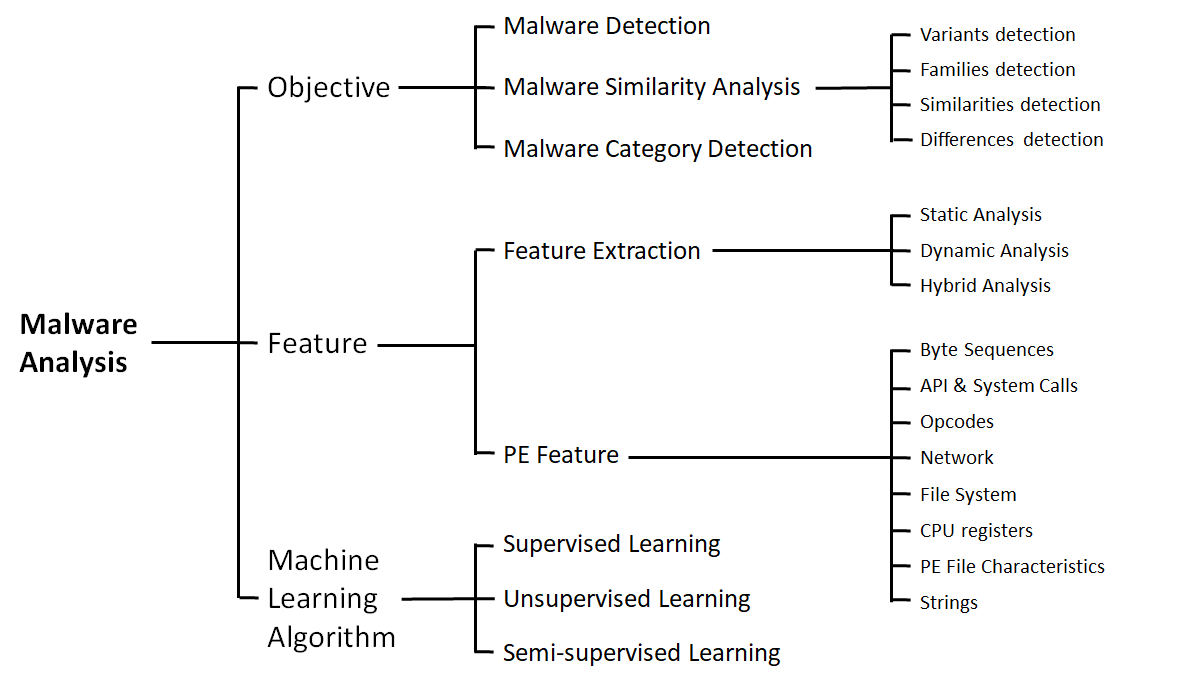
\includegraphics[width=0.6\textwidth, center]{components/images/SotA.png}
	\label{fig:sota}
    \captionsetup{justification=centering,margin=1cm}
    \captionof{figure}{Taxonomie din Articolul Citat}
\end{frame}

\extras{
    \begin{frame}{Motivație II} \pause
    	\begin{itemize}
    		\item Oferirea numai a unor soluții teoretice, metodologii \pause
    		\item Nu și a unora practice, programe sau biblioteci de cod
    	\end{itemize}
    \end{frame}
}